\subsection{体积的概念与公理}\label{subsec:2-7}

在生产建设和科学实验中,经常会遇到关于物体体积的问题,这些问题与各种几何体的体积有关。
这一节我们就来研究这些几何体的体积问题。

几何体占有空间部分的大小叫做它的\zhongdian{体积}。

同度量长度、面积一样,要度量一个几何体的体积,首先要选取一个单位体积作为标准,
然后求出几何体的体积是单位体积的多少倍,这个倍数就是这个几何体的体积的数值。
通常取棱长等于单位长度(例如 1 cm、1 m 等)的正方体的体积作为\zhongdian{体积单位}(图 \ref{fig:ltjh-2-57})。

\begin{figure}[htbp]
    \centering
    \begin{minipage}[b]{5cm}
        \centering
        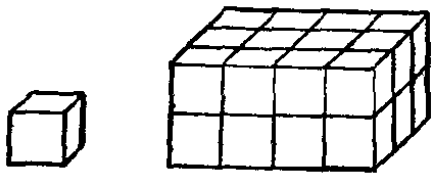
\includegraphics[width=5cm]{../pic/ltjh-ch2-57.png}
        \caption{}\label{fig:ltjh-2-57}
    \end{minipage}
    \qquad
    \begin{minipage}[b]{9cm}
        \centering
        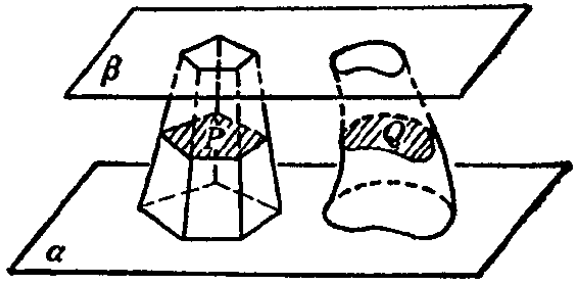
\includegraphics[width=9cm]{../pic/ltjh-ch2-58.png}
        \caption{}\label{fig:ltjh-2-58}
\end{minipage}
\end{figure}


作为推算体积的基础,我们把下面的两个事实当作公理。

\begin{gongli}[公理5][gl:5]
    长方体的体积等于它的长、宽、高的积。
    \begin{center}
        \framebox[10em]{$\bm{V_\text{长方体} = abc}$。}
    \end{center}
\end{gongli}

从这个公理,可以直接得到下面的推论:

\begin{tuilun}[推论1][tl:5-1]
    长方体的体积等于它的底面积 $\bm{S}$ 和高 $\bm{h}$ 的积。
    \begin{center}
        \framebox[10em]{$\bm{V_\text{长方体} = Sh}$。}
    \end{center}
\end{tuilun}


\begin{tuilun}[推论2][tl:5-2]
    正方体的体积等于它的棱长 $\bm{a}$ 的立方。
    \begin{center}
        \framebox[10em]{$\bm{V_\text{正方体} = a^3}$。}
    \end{center}
\end{tuilun}

\begin{gongli}[公理6][gl:6]
    夹在两个平行平面间的两个几何体,被平行于这两个平面的任意平面所截,
    如果截得的两个截面的面积总相等,那么这两个几何体的体积相等。
\end{gongli}

图 \ref{fig:ltjh-2-58} 表示,夹在平行平面 $\alpha$、$\beta$ 之间的两个形状不同的几何体,
被平行于平面 $\alpha$、$\beta$ 的任意一个平面所截,如果截面 $P$ 和 $Q$ 的面积总相等,
那么它们的体积一定相等。

例如,取一摞书或一摞纸张堆放在桌面上,将它如图 \ref{fig:ltjh-2-59} 那样改变一下形状,
这时高度没有改变,每页纸的面积也没有改变,因而这摞书或纸张的体积与变形前相等。

我国古代数学家祖暅,早在公元五世纪,就在实践的基础上,总结出这个\hyperref[gl:6]{公理},
并首先使用这个公理证明了球的体积公式,因而我们把它叫做\zhongdian{祖暅原理}\mylabel{zgyl}[祖暅原理]。
在欧洲直到十七世纪,才有意大利的卡发雷利提出这个事实。

用以上两个公理作基础,我们就可以求出柱、锥、台、球等的体积。

\begin{figure}[htbp]
    \centering
    \begin{minipage}[b]{9cm}
        \centering
        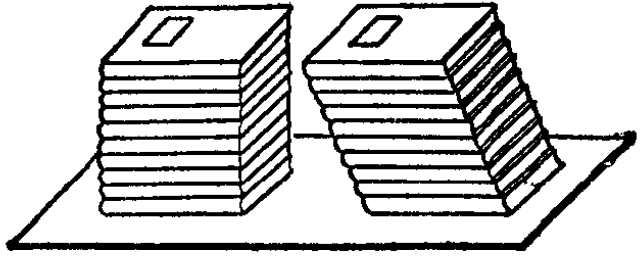
\includegraphics[width=9cm]{../pic/ltjh-ch2-59.png}
        \caption{}\label{fig:ltjh-2-59}
    \end{minipage}
    \qquad
    \begin{minipage}[b]{5cm}
        \centering
        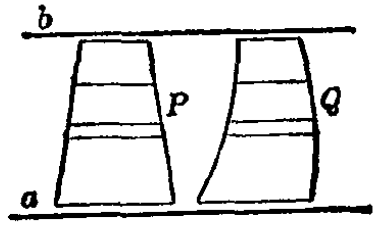
\includegraphics[width=5cm]{../pic/ltjh-ch2-subsec7-lx-02.png}
        \caption*{(第 2 题)}
    \end{minipage}
\end{figure}

\begin{lianxi}

\xiaoti{用棱长为 1 的正方体的体积作为体积单位,图 \ref{fig:ltjh-2-57} 中长方体体积的数值为 24。
    假如将体积单位改用棱长为 2 的正方体的体积,这个长方体的体积变为多少?为什么?
}

\xiaoti{把夹在两条平行线间的两个平面图形的面积相等的条件,用祖暅原理的形式叙述出来。
    并根据矩形面积公式,求平行四边形的面积公式。
}

\end{lianxi}

